\documentclass[letterpaper]{article}
\usepackage{aaai}
\usepackage{times}
\usepackage{helvet}
\usepackage{courier}
\frenchspacing
\setlength{\pdfpagewidth}{8.5in}
\setlength{\pdfpageheight}{11in}
\pdfinfo{
/Title (Calibration-Free BCI Based Control)
/Author (Jonathan Grizou, I\~naki Iturrate, Luis Montesano, Manuel Lopes, Pierre-Yves Oudeyer)}
\setcounter{secnumdepth}{0}  
% \setlength\titlebox{2.5in}

%% package we used
\usepackage{algorithm}
\usepackage{algorithmic}
    
\usepackage{amsmath}
\usepackage{amsfonts}
\usepackage{amssymb}
    
\usepackage{graphics}
\usepackage{graphicx}

\usepackage{verbatim}

\usepackage{epstopdf}
\usepackage{caption}
\usepackage{subcaption} 
\renewcommand{\L}{\mathcal{L}}

\newcommand{\ww}{0.9}

\begin{document}

\title{Calibration-Free BCI Based Control}
\author{Jonathan Grizou \\ Inria Bordeaux Sud-Ouest, France \\ jonathan.grizou@inria.fr
\And I\~naki Iturrate \\ CNBI, EPFL, Switzerland \\ inaki.iturrate@epfl.ch
\AND Luis Montesano \\ I3A, Univ. of Zaragoza, Spain \\ montesano@unizar.es
\And Pierre-Yves Oudeyer \\ Inria Bordeaux Sud-Ouest, France \\ pierre-yves.oudeyer@inria.fr
\And Manuel Lopes \\ Inria Bordeaux Sud-Ouest, France \\ manuel.lopes@inria.fr}

\maketitle

\begin{abstract}
\begin{quote}
Recent works have explored the use of brain signals to directly control virtual and robotic agents in sequential tasks. So far in such brain-computer interfaces (BCI), an explicit calibration phase was required to build a decoder that translates raw electroencephalography (EEG) signals from the brain of each user into meaningful instructions.
%
This paper proposes a method that removes the calibration phase, and allows a user to control an agent to solve a sequential task.
%
The proposed method assumes a distribution of possible tasks, and infers the interpretation of EEG signals and the task by selecting the hypothesis which best explains the history of interaction. 
%
We introduce a measure of uncertainty on the task and on the EEG signal interpretation to act as an exploratory bonus for a planning strategy. This speeds up learning by guiding the system to regions that better disambiguate among task hypotheses.
%
We report experiments where four users use BCI to control an agent on a virtual world to reach a target without any previous calibration process.
\end{quote}
\end{abstract}

\section{Introduction}

EEG-based brain-computer interfaces (BCI) have been used successfully to control different devices, such as robotic arms and simulated agents, using self-generated (e.g. motor imagery) and event-related potentials signals (see \cite{millan2010combining} for a review). 
%
Error-related potentials (ErrPs) are one kind of event-related potential appearing when the user's expectation diverges from the actual outcome \cite{Falkenstein00}. Recently, they have been used as feedback instructions for devices to solve a user's intended task \cite{chavarriaga2010learning,iturrate13}.

As in most BCI applications, ErrP-based BCI requires a calibration phase to learn a decoder (e.g. a classifier) that translates raw EEG signals from the brain of each user into meaningful instructions. This calibration is required due to specific characteristics of the EEG signals: non-stationary nature \cite{vidaurre2011toward}, large intra- and inter-subject variability \cite{Polich1997}, and variations induced by the task \cite{IturrateErrP13}. The presence of an explicit calibration phase, whose length and frequency is hard to tune and is often tedious and impractical for users, hinders the deployments of BCI applications out of the lab. Thus, calibration free methods are an important step to apply this technology in real applications \cite{millan2010combining}.

Despite the importance of calibration-free BCI, there are only few related works. For long term operation using sensory-motor rhythms, it is possible to adapt the decoder online \cite{vidaurre2010towards}. In invasive BCI, \citeauthor{Orsborn2012} (\citeyear{Orsborn2012}) proposed a method to learn from scratch and in closed loop a decoder for known targets using pre-defined policies to each target.  However, the approach needs a warm-up period of around 15 minutes. For P300 spellers, Kindermans et al. proposed a method to auto-calibrate the decoder by exploiting multiple stimulations and prior information \cite{kindermans2012bayesian,kindermans2012p300,tangermann2013zero}. They exploit the particular fact that only one event out of six encodes a P300 potential in the speller paradigm.

Our main contribution is a calibration-free BCI method that infers simultaneously and seamlessly an EEG decoder of error-related potentials while controlling a device to achieve a sequential task. The core idea of the method is to assume a distribution of possible tasks, and infer the interpretation of EEG signals and the task by selecting the hypothesis which best explains the history of interaction. This inference can be continuously run and updated as new data comes in, which removes the need for an explicit calibration.

This method is inspired from our previous work \cite{grizou2013robot} which considered a robotic setting and speech utterances as feedback signals. In the current work we improve the algorithm formalism, the robustness to noisy high-dimensional signals (e.g.\ EEG), and show that it is possible to use model-based planning relying on the uncertainty about the task and the feedback signals interpretation to explore the space efficiently while learning.

We also present an evaluation of this method with online experiments where four users control an agent in a virtual world. The results show that the proposed method allows to learn a good signal decoder and solve the task efficiently without any explicit calibration. Offline experiments show that our unsupervised trained decoder achieves similar performances than calibration based systems and illustrate the benefits of our planning strategy for speeding up learning.

\section{Calibration-Free BCI Based Control}

\subsection{BCI control based on feedback signals}

BCI control based on feedback signals differs from classical brain-computer interfaces in the sense that the user does not actively deliver commands to the device, but only delivers feedback about actions performed by the device \cite{chavarriaga2010learning,iturrate13}. In this setting, the device needs to actively execute a sequence of several actions to solve the task and to be able to learn an intelligent behavior from the feedback. This idea can be seen as a shared control strategy \cite{millan2010combining}, where both the user and the device help each other to solve a task.

Essentially, this BCI control follows an iterative sequential process where the device performs an action which is in turn assessed by the user. This assessment will elicit potentials into the user's brain that can be recorded using EEG and will be different for ``correct'' and ``wrong'' assessments. The potentials elicited in the user's brain after performing assessments are called error-related potentials \cite{FerrezErrores}. After a calibration phase and once a usable decoder of these signals is available, user's assessments can be translated into (normally binary) feedback, which the device can use to adapt its behavior. 

This control based on user's assessments decoded from brain signals can be exemplified for a reaching task, where the user wants to reach a target position unknown by the system. The device performs several discrete actions (e.g. moving left or right), and learns from the feedback given by the user. After several iterations, if the meanings of the EEG assessment signals provided by the users are known, the device can infer which is the user's desired position and how to reach it. The following section explains how we can achieve similar performances without knowing the brain signal decoder beforehand. We will use the term ``virtual label'' or ``label'' to denote the interpretation of a given EEG signal as a feedback instruction (e.g. ``correct'' or ``wrong'').

\subsection{Simultaneous Estimation of Task and Signal Model}
\label{sec:Algorithm}
\begin{figure}[!ht]
\centering
    \begin{tabular}{c|c|c}
        \begin{subfigure}[t]{0.29\columnwidth}
            \begin{flushleft}
            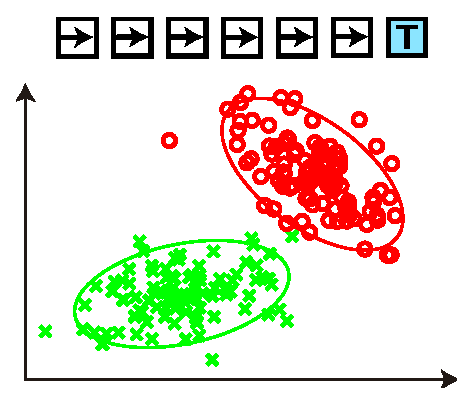
\includegraphics[width=\columnwidth]{img/GM1}
            \caption{}
            \label{fig:GM1}
            \end{flushleft}
        \end{subfigure}
        &
        \begin{subfigure}[t]{0.29\columnwidth}
            \begin{center}
            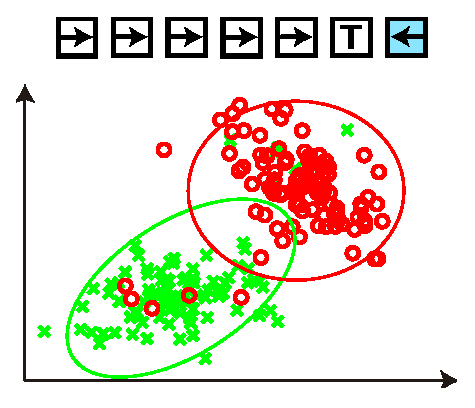
\includegraphics[width=\columnwidth]{img/GM2}
            \caption{}
            \label{fig:GM2}
            \end{center}
        \end{subfigure}
        &
        \begin{subfigure}[t]{0.29\columnwidth}
            \begin{flushright}
            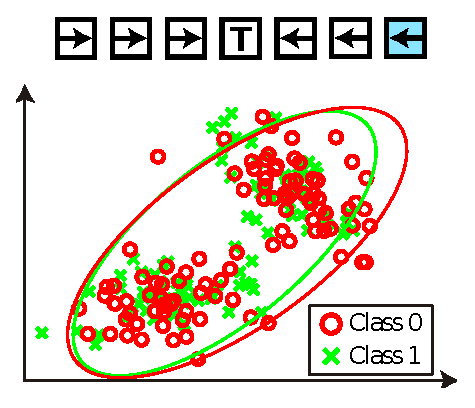
\includegraphics[width=\columnwidth]{img/GM3}
            \caption{}
            \label{fig:GM3}
            \end{flushright}
        \end{subfigure}
    \end{tabular}
\caption[]{Representation of inferred signal labels for a 1D grid world in function of the hypothesized task. Three task hypotheses are displayed in column from left to right [(a),~(b),~(c)]. On top is a 1D grid world with the hypothetic target state marked with a T letter. Notice that this hypothetic target is different for each of the three hypotheses. The arrows in each cell indicates what action should elicit a positive feedback, i.e.\ the optimal policy with respect to the hypothetic target. The user intended target is shown as the shaded blue state at the right extremity of the 1D world. Note that the system does not have access to this information. The correct hypothesis is the one on the Left [(a)] where the T state is the same as the shaded blue state.
Below the 1D grid world, the signals received from the user are represented in a 2D feature space. They represent the user assessment signals of the past history of device's actions (e.g.\ moving randomly left and right). Our algorithm assigns virtual labels (green for ``correct'' and red for ``wrong'') to those signals with respect to their respective hypothetic target. Notice that the data points are the same for all three hypotheses, only their respective labels differ.
With the virtual labels being assigned, we can compute the corresponding 2D Gaussian distributions estimates for each class (shown as colored ellipses) and each hypothesis. While for the correct hypothesis [(a)] the Gaussian distributions shows a large separability, the overlap increases as the hypothetic target (T) moves away from the real (blue shaded) one [(b), (c)]. This property can be exploited to estimate the correct hypothesis and the model generating the signals.}
\label{fig:GM}
\end{figure}
%
This section formalizes the problem of executing a task when the mapping between raw EEG signals to a discrete label among a set of pre-defined labels is unknown. The main idea is depicted in Figure~\ref{fig:GM} for a toy 1D example. The user wants the device to reach the right-most state. For each device's action, he provides a feedback signal which encode whether the action executed is ``correct'' or ``wrong'' according to the intended target. Such signals are generated from an underlying model which maps a binary label (``correct'' or ``wrong'') to a continuous signal. However, neither the user's desired target nor the labels associated to the user's feedback signals are known.

Considering that we can define a finite set of task hypotheses (e.g. reaching one of a finite number of states), we can infer the labels that should be provided by the user with respect to each hypothesis. Then, given a particular interaction history, it is possible to compute a different signal decoder for each task hypothesis. The key point is that only the correct hypothesis will assign the correct labels to all feedback signals (Figure~\ref{fig:GM1}), while the other hypotheses will gradually mix both classes as the hypothetic target gradually differs more from the correct one (Figure~\ref{fig:GM2}~and~\ref{fig:GM3}). Therefore, the hypothesis which provides the decoder with best accuracy and compactness can be selected as the most probable one. In the remainder of this section we show how this property can be exploited to estimate the target and the model generating the feedback signals.

Formally, we represent the problem as a discrete or continuous set of states $s \in S$,  a finite set of possible actions $a \in A$, and a set of possible tasks, or targets, for which the system is able to plan the best sequence of actions. In the 1D example in Figure~\ref{fig:GM}, the state space is composed of seven discrete states, and the agent can perform unitary directional actions, i.e. move one cell left or right. During an interactive learning session, the agent will proactively perform actions which will in turn be evaluated as ``correct'' or ``wrong'' by the user with respect to the desired target state on the grid. In our case the feedback signals are error-related potentials measured in the brain activity of the subject.

Let $e_i\in \mathbf{R}^n$ denote the feature vector of the EEG measurements obtained at iteration $i$ after the device performed action $a_i$ in state $s_i$. The label $z_i\in\{c,w\}$ of each feedback signal belongs to one of two classes (``correct'' or ``wrong'').
%
Following \citeauthor{blankertz2010single} (\citeyear{blankertz2010single}), we will model the EEG signals using independent multivariate normal distributions for each class ($\mathcal{N}(\mu_c, \Sigma_c)$ and $\mathcal{N}(\mu_w, \Sigma_w)$). We will denote by $\theta$ this set of parameters $\{\mu_c, \Sigma_c,\mu_w, \Sigma_w\}$.

We assume the system has access to a set of task hypotheses $\xi_1,\ldots,\xi_T$ which includes the task the user wants to solve. We do not make any particular assumption on how the task is represented but we assume that for each particular task $\xi$ we are able to compute a policy $\pi_\xi$ which represents the probability of choosing a given action $a$ in state $s$, $\pi_{\xi}(s,a) = p(a|s,\xi)$. As mentioned above, these are the policies that, conditioned on the task, provide labels to the feedback signals of a state-action pair (e.g. in a reaching task, progressing towards the goal will generate ``correct'' feedback while moving apart from it will generate ``wrong''feedback).

The method aims to infer which task $\hat{\xi}$ the user wants to solve based on the user's feedback signals extracted from EEG measurements collected while the agent executes some actions. Following the analysis of Figure~\ref{fig:GM}, a sensible option to estimate the task is to measure the coherence of the signal model for each possible task using the virtual labels provided by the target policy. In other words, the best $(\xi,\theta)$ pair provides the lowest predictive error on the observed signals $p(e|s,a,\xi,\theta)$, which themselves were collected in the recent history of interaction. One possible way of solving this problem is to maximize the expected classification rate:
%
\begin{eqnarray}
\hat{\xi},\hat{\theta}&=& \arg\max_{\xi,\theta} E_e\left[ \delta(z(s,a,\xi), z(e,\theta)) \right]
\end{eqnarray}
%
where $\delta()$ is an indicator function, $z(s,a,\xi)$ is the label (correct or wrong) corresponding to the execution of action $a$ in state $s$ under task $\xi$ and $z(e,\theta)$ is the label provided by classifying the EEG signal $e$ under the Gaussian classifier parameterized by $\theta$. The expected classification rate ($Ecr$) can be explicitly written dependent on the task and decoder model:
%
\begin{eqnarray}
\lefteqn{Ecr\left( \delta(z(s,a,\xi), z(e,\theta)) \right) =}\nonumber\\
 &=& \sum_{k \in \{c,w\}} p(z=k|s,a,\xi) p(z=k|e,\theta)
\label{eq:ecr} 
\end{eqnarray}
%
where $p(z=k|s,a,\xi)$ represents the probability of the user assigning label $k$ when assessing action $a$ in state $s$ according to task $\xi$. We add a noise term to cope with those situations where the user assessment may be wrong. The model for probability of correct assessment is then:
%
\begin{equation}
    p(z=c|s,a,\xi) = \begin{cases}
                           1-\alpha           & if~a = \arg\max_{a} \pi_{\xi}(s,a)\\
                           \alpha             & \text{otherwise}\\
                       \end{cases}
\end{equation}
%
with $\alpha$ modeling the assessment error rate of the user, which was set to $0.1$ for our experiments.

Finally, the term $p(z=k|e,\theta)$ is just the probability that the signal $e$ belong to class $k$ under the Gaussian model provided by $\theta$ and is given by:
%
\begin{eqnarray}
    p(z=k|e,\theta) &=& 
                \frac{p(e|z=k, \theta)p(z = k)}{\sum_{l \in \{c,w\}}{p(e|z=l,\theta)p(z=l)}}\nonumber\\
                 &=& \frac{\mathcal{N}(e|\mu_k, \Sigma_k)p(z = k)}{\sum_{l \in \{c,w\}}{\mathcal{N}(e|\mu_l, \Sigma_l)p(z=l)}}
    \label{eq:dev}
\end{eqnarray}
%
As we do not have a priori knowledge on the user intended meaning, we assume that it is equiprobable $p(z = c) = p(z = w)$. We will factorize the optimization process using the fact that given a task $\xi$, the estimation of $\theta$ under the Gaussian model is straightforward. It basically requires to compute the maximum-likelihood estimate $\theta^{ML}_{\xi}$ using the labels associated to target $\xi$. We could also consider a prior distribution on the parameters and update it with new observations. Using the labels of target $\xi$, the estimation of $\theta$ under the Gaussian model described above simply returns to the computation of the posterior mean $\mu_z$ and covariance $\Sigma_z$ for each class $z \in \{c, w\}$. In order to avoid numerical problems when estimating the covariance for a low number of examples, a regularization term was applied to penalize very large and very small eigenvalues \cite{friedman1989regularized}:
%
\begin{eqnarray}
\Sigma_z = (1-\lambda)\Sigma_z + \lambda \frac{trace(\Sigma_z)}{n} \textbf{I}_n
\end{eqnarray}
%
with n the feature dimension, $\textbf{I}_n$ the identity matrix of size $n$, and $\lambda$ the regularization term which was set to $0.5$ for our experiments. An automatic adaptation of the regularization could also be considered \cite{ledoit2004well}.

Using equation~\ref{eq:ecr} to estimate the expected classification rate is difficult because we ideally want to estimate it on future, never observed, data. A possible solution is to use cross-validation or bootstrapping methods using the available data. However, for small amounts of data, these methods result in estimates with high variance \cite{bengio2004no} and computational cost.

Alternatively, we propose to use another approximation of the expected classification rate, the Bhattacharyya coefficient. This coefficient has been related to the classification error of Gaussian models \cite{Kailath67} and is inversely proportional to the classification rate. Although there is no analytical relation between the coefficient and the classification rate, it is possible to derive bounds and good empirical approximations \cite{lee2000bayes}.
%
The Bhattacharyya coefficient $\rho \in [0,1]$ between the Gaussian distributions associated to label ``correct'' ($\mathcal{N}(\mu_c, \Sigma_c)$) and ``wrong'' ($\mathcal{N}(\mu_w, \Sigma_w)$) is:
%
\begin{eqnarray}
\rho = e^{-D_B(\theta)}
\end{eqnarray}
%
where $D_B$ is the Bhattacharyya distance:
$D_B(\theta)=$\\$\frac{1}{8}(\mu_c-\mu_w)^T(\frac{\Sigma_c+\Sigma_w}{2})^{-1}(\mu_c-\mu_w)+\frac{1}{2}ln\left(\frac{det(\frac{\Sigma_c+\Sigma_w}{2})}{\sqrt{det\Sigma_c det\Sigma_w}}\right)$. 

Finally, we approximate the expected classification rate as: 
\begin{eqnarray}
Ecr \propto 1 - \rho
\end{eqnarray}


\subsection{Confidence on Target Estimation}

Now that we have an estimation of the expected classification rate, we need to take a decision with respect to which task is the one intended by the user. To do so we should compare the expected classification rate of every task hypothesis $\xi_t$ with $t \in \{1, \ldots, T\}$. The hypothesis whose associated model has the highest expected classification rate, i.e.\ the lowest value of $\rho$, is expected to be the one intended by the user, however it is meaningless to define an absolute threshold on the value of the expected classification rate itself. Indeed, different people generate different signals which result in classifiers of different qualities. To bypass this problem we rely on a voting system where we attribute each hypothesis $\xi_t$ a weight that is updated at every iteration.

We rely on a pseudo-likelihood metric that for each hypothesis $\xi_t$ accumulate expected classification rate over time:
%
\begin{eqnarray}
\L(\xi_t) = \prod_{i = 1}^{N} 1 - \rho_i^{\xi_t}
\end{eqnarray}
%
with N the current number of iteration and $\rho_i^{\xi_t}$ the Bhattacharyya coefficient associated to task $\xi_t$ using all data up to time $i$. By normalizing the pseudo-likelihood values between every hypothesis, we obtain what can be viewed as the probability of each target:
%
\begin{eqnarray}
p(\xi_t) = \frac{\L(\xi_t)}{\sum_{u \in \{1, \ldots, T\}} \L(\xi_u)}
\end{eqnarray}
%
Once a target reaches a probability threshold $\beta$ we consider it as being the correct one, i.e.\ the one intended by the user. We used $\beta = 0.99$.

\subsection{Estimation of further Tasks and Online Re-Estimation of Signal Model}
\label{sec:AlgReUse}

Once we have identified a first task, the user can change his desired target and our system has to identify the new target. However, the model of the feedback signals does not change and does not have to be re-learned from scratch. Indeed, once the system has correctly identified a task, it is possible to reuse acquired data by assigning to all the previously collected signals the labels associated to the previously estimated task. 

The use of the Bhattacharyya coefficient provides a simple and efficient way to estimate a first target from scratch (when the number of examples is small) but does not allow a fast adaptation to new targets as the majority of collected signals now belong to the previous task. To avoid this problem we compute a classifier (e.g. a Gaussian Bayes classifier), and use it similarly to calibrated approaches in BCI. For this we factorize the joint distribution:
%
\begin{eqnarray}
p(\xi_t, \theta \mid D^{\xi_t}_i) & \propto & p(\xi_t \mid D^{\xi_t}_i)p(\theta \mid \xi_t, D^{\xi_t}_i)
\end{eqnarray}
%
where $D^{\xi_t}_i$ contains all the quadruplet $(e_i,s_i,a_i,z_i)$ up to time $i$, with the associated labels $z_i$ assigned with respect to task $\xi_t$. The factorization makes explicit that given the task $\xi_t$, the distribution $p(\theta \mid \xi_t, D^{\xi_t}_i)$ can be easily evaluated using the labels of each target. We approximate this posterior using the maximum likelihood point estimate $\theta^{ML}_{\xi_t}$ per target. For the term $p(\xi_t \mid D^{\xi_t}_i)$, we use a recursive Bayes filter:
%
\begin{eqnarray}
p(\xi_t \mid D^{\xi_t}_i) &\propto & p(e_i \mid \xi_t, (s,a)_i,D^{\xi_t}_{i-1})p(\xi \mid D^{\xi_t}_{i-1}) \nonumber\\
& \approx & p(e_i\mid \theta^{ML}_{\xi_t})p(\xi_t \mid D_{i-1}).
\label{eq:taskprob}
\end{eqnarray}
%
Notice that we are keeping a different symbol model  $\theta^{ML}_{\xi_t}$  for each possible target $\xi_t$, the maximum likelihood estimation needs to be done in relation to a dataset $D^{\xi_t}_{i-1}$ which include the expected labels of target $\xi_t$ up to time $i-1$. 

We use the same threshold mechanism as described in previous subsection to decide whether or not a task can be considered the correct one. Whenever a task is identified, its labels are transferred to the quadruplets $D^{\xi_t}_{i}$ of all the other tasks to correct the prior for the next step with the right labels. This scheme performs a long term adaptation of $\theta$ to accommodate slight variations of EEG such as non-stationarities or variations induced by the task. 

However, as tasks are identified, the prior becomes more informative and the adaptation may have problems to cope with drastic changes such as strongly modifying the signals. To handle this problem, we chose to limit the size of the prior through the use of a sliding window on past iterations which allows to estimate a moving average of parameters $\theta$. In practice, we limited $D^{\xi_t}_{i}$ to the last $250$ elements.

\subsection{Planning}
\label{alg:planning}

Our algorithm is able to identify a task among a set of possible tasks. To do so it has to explore regions allowing to disambiguate among task hypotheses. There are several efficient model-based reinforcement learning exploration methods that add an exploration bonus for states that might provide more learning gains. Several theoretical results show that these approaches allow to learn tasks efficiently \cite{brafman2003r,kolter2009near}. We define an uncertainty measure and use model-based planning to select sequences of actions that guide the agent towards states that better identify the desired task.

Our algorithm is based on comparing the expected classification rate between different task hypotheses. Therefore, to disambiguate between hypotheses, it has to collect data which are likely to affect differently the dataset quality of competing hypotheses. As we have access to the optimal policies of each task, we can choose for a given task an action in a given state and predict to receive a ``correct'' or ``wrong'' label. Such label is linked to a signal generation model (parameterized by $\theta^{ML}_{\xi_t}$) which differs from task to task, and to the optimal action at that particular state. A state-action pair where the optimal actions and the signal models are the same for all hypotheses is unlikely to tell them apart and will be less informative that any other state-action where either optimal actions or signal models differ between hypotheses.

Thus, we define a measure of global uncertainty $U(s,a)$ that is higher when, for a given state-action, there is a high incongruity between either optimal actions or signal models. For this we compute a similarity matrix $S$ where each element $S_{ij}(s,a)$ corresponds to the similarity of the distributions of signals associated to the expected label from tasks $i$ and $j$ if action $a$ is performed in state $s$. The final uncertainty value $U(s,a)$ is computed as the opposite of the weighted sum of the similarity matrix elements:
%
\begin{eqnarray}
U(s,a) &=& - \sum_{i = 1}^{T} \sum_{j = 1}^{T} S_{ij}(s,a) p(\xi_i)p(\xi_j)
\end{eqnarray}
%
Computing the similarity between two Gaussian distributions for all state-action pairs was not feasible in real time. In order to improve computation efficiency we do not rely on a precise metric between Gaussian distributions and only consider the similarity between their means (empirical tests did show that this approximation does not impact the results).

Computed for each state and action, this measure is then used as an exploration bonus, whereas we switch to a pure exploitation of the task after reaching the desired confidence level~$\beta$.

\section{Experimental Protocol and Results}
\label{sec:results}

\subsection{Control task}
We consider a 5x5 grid world, where an agent can perform five different discrete actions: move up, down, left, right, or a target-reached action. The user goal is to teach the agent to reach one, yet unknown to the agent, of the $25$ discrete states which represent the set of possible tasks (i.e. one task per possible target state). We thus consider that the agent has access to 25 different task hypotheses. We use \textit{Markov Decision Processes} (MDP) to represent the problem \cite{sutton1998reinforcement}. From a given task $\xi$, represented as a reward function, we can compute the corresponding policy $\pi_{\xi}$ using, for instance, Value Iteration \cite{sutton1998reinforcement}. 

\subsection{EEG-based feedback signals}

EEG signals were recorded with a gTec system (2 gUSBamp amplifiers) with 32 electrodes distributed according to the 10/10 international system, with the ground on FPz and the reference on the left earlobe. The EEG signals were digitized with a sampling frequency of $256$ Hz, common-average-reference (CAR) filtered and band-pass filtered at $[0.5, 10]$ Hz. 

During operation, the role of the users was to mentally assess the agent's actions as correct or wrong with respect to a selected target, obtaining this way error-related potentials. Previous studies have demonstrated that these signals can be detected online \cite{FerrezErrores}. Following these studies, features were extracted from two fronto-central channels (FCz and Cz) within a time window of $[200,700]$ ms ($0$ ms being the action onset of the agent) and downsampled to $32$ Hz. This leaded to a vector of $34$ features that was the input for our system.

\subsection{Calibration-Free Online BCI Control}

This experiment evaluates if we can identify the task desired by the user even without an explicit calibration phase and without prior knowledge of the brain signals. The experiments were conducted with four subjects (aged between $25$ and $28$). Each subject was asked to mentally assess the agent's actions with respect to a given target. The system was not calibrated to decode the user EEG signals beforehand. Each subject performed $5$ runs, for each run a new target was randomly selected and provided to the user. There was an action every three seconds. Each run lasted $200$ actions, and the time between runs was around one minute.

The algorithm was able to identify the correct target for all runs of all the subjects, see Figure~\ref{fig:online_results}. There are strong variations among subjects but we note that our system identified each task in less iterations than a normal calibration phase requires (between 300 and 600 examples depending on the user performance \cite{chavarriaga2010learning,iturrate2010single}).

\begin{figure}[!htbp]
    \centering
    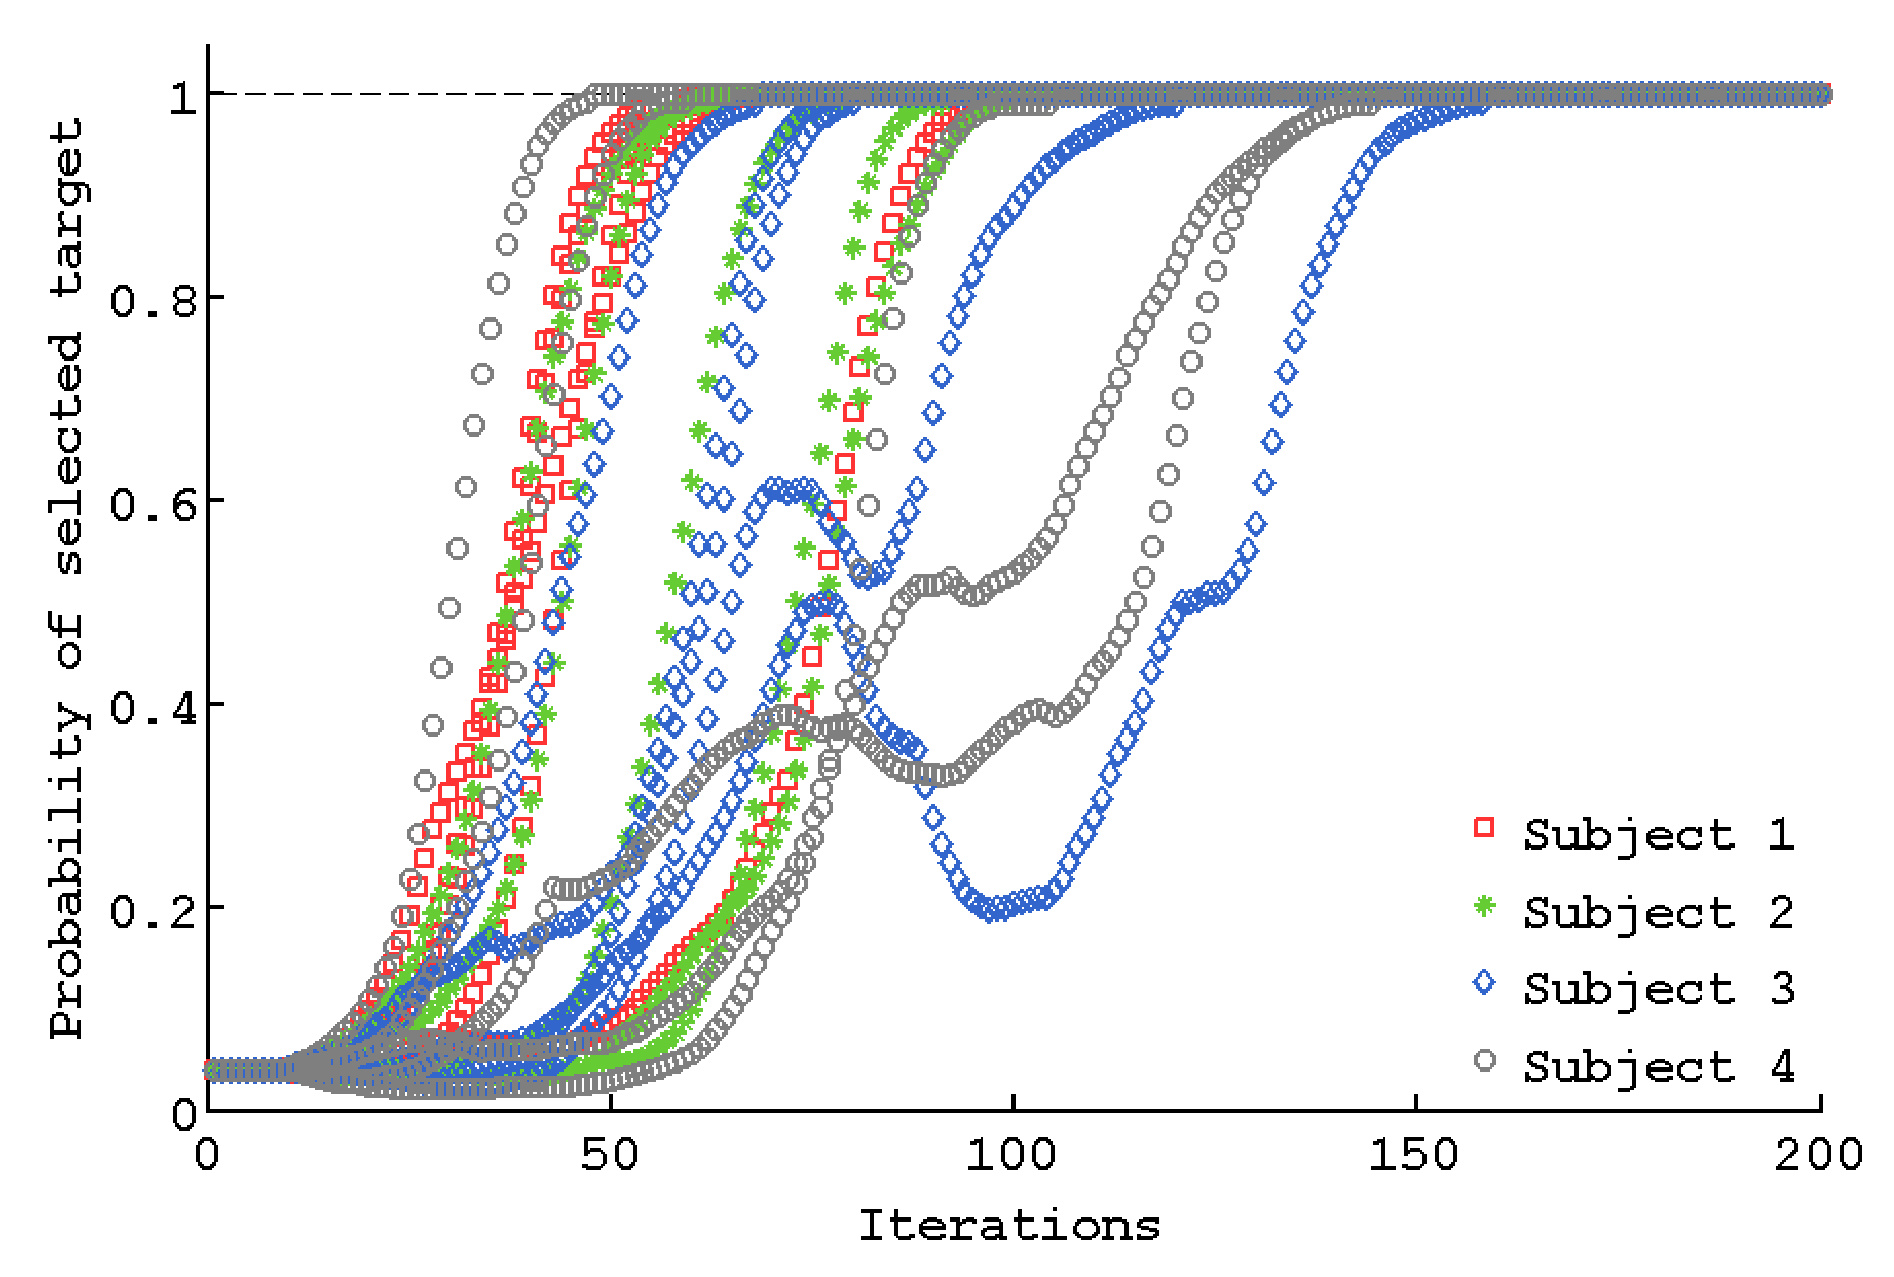
\includegraphics[width=\ww\columnwidth]{img/plot_realevolution}    
    \caption{Results from the online experiment: Evolution of the probability of the correct task for each subject and run. The algorithm was able to identify the correct target for each subjects and runs in less than 200 iterations.}
    \label{fig:online_results} 
\end{figure}

Table~\ref{ch6tab:steps} shows for each subject and run the number of iterations needed to reach the confidence threshold for the subject selected target.

On average, the number of iterations needed to identify the target was of 85 $\pm$ 32.

\begin{table}[!ht]
\centering
\begin{footnotesize}
\begin{tabular}{r|rrrrr|r}
    %\toprule
    & \textbf{Run1} & \textbf{Run2} & \textbf{Run3} & \textbf{Run4} & \textbf{Run5} & \textbf{mean$\pm$std} \\\hline
    %\midrule
    \textbf{S1} & 95 & 62 & 56 & 60 & 64 & 67 $\pm$ 16 \\
    \textbf{S2} & 89 & 77 & 98 & 60 & 62  & 77 $\pm$ 17 \\
    \textbf{S3} & 68 & 80 & 118 & 76 & 157 & 100 $\pm$ 37 \\
    \textbf{S4} & 98 & 142 & 57 & 142 & 47 & 97 $\pm$ 45 \\
    %\bottomrule
\end{tabular}
\end{footnotesize}
  \caption{Results from the online experiment: Number of iterations needed to identify the correct target for each subject and run. On average, the number of iterations needed to identify the target was of 85 $\pm$ 32.}
  \label{ch6tab:steps}
\end{table}

\subsection{Algorithm Offline Analysis}

The objective of the offline analysis is to study the impact of our exploration method and evaluate if the classifier learned from scratch with our algorithm can be reused for learning new tasks. Finally we want to evaluate how robust the system is to abrupt changes in the signal properties. For these experiments, to ensure we have sufficient data to achieve statistically significant results, we rely on a large dataset of real EEG data. We used a dataset from \cite{IturrateErrP13}, which covers ten subjects that performed two different control problems (denoted $T1$ and $T2$). The role of the users was similar (assess the agent's actions), but the problems differs in the state-action space size and visual representations. For each subject, $T1$ was composed of 1800 assessments, and $T2$ of 1200. Despite the fact that both problems elicit error-related potentials, the EEG signals presented significant differences \cite{IturrateErrP13}.

For each subject, and each dataset ($T1$ and $T2$), we simulated $20$ runs of $400$ iterations following the control task. Each time the device performed an action, we sampled the dataset using the ground truth labels corresponding to the correct task and then removed the chosen signal from it. After a first task was identified, and following our approach, we continued running the system to identify new tasks. 

We present most of the results in terms of the quality of the dataset, measured as the classification accuracy that a calibrated brain signal classifier would obtain. Results vary strongly between subjects and we will see that it is a direct consequence of the difficulty of finding a classifier with high accuracy. 

\paragraph{Planning Methods}
We compared the average number of steps (with maximum values of $400$ steps) needed to identify the first task when learning from scratch with different planning methods.

\begin{figure}[!ht]
    \centering
    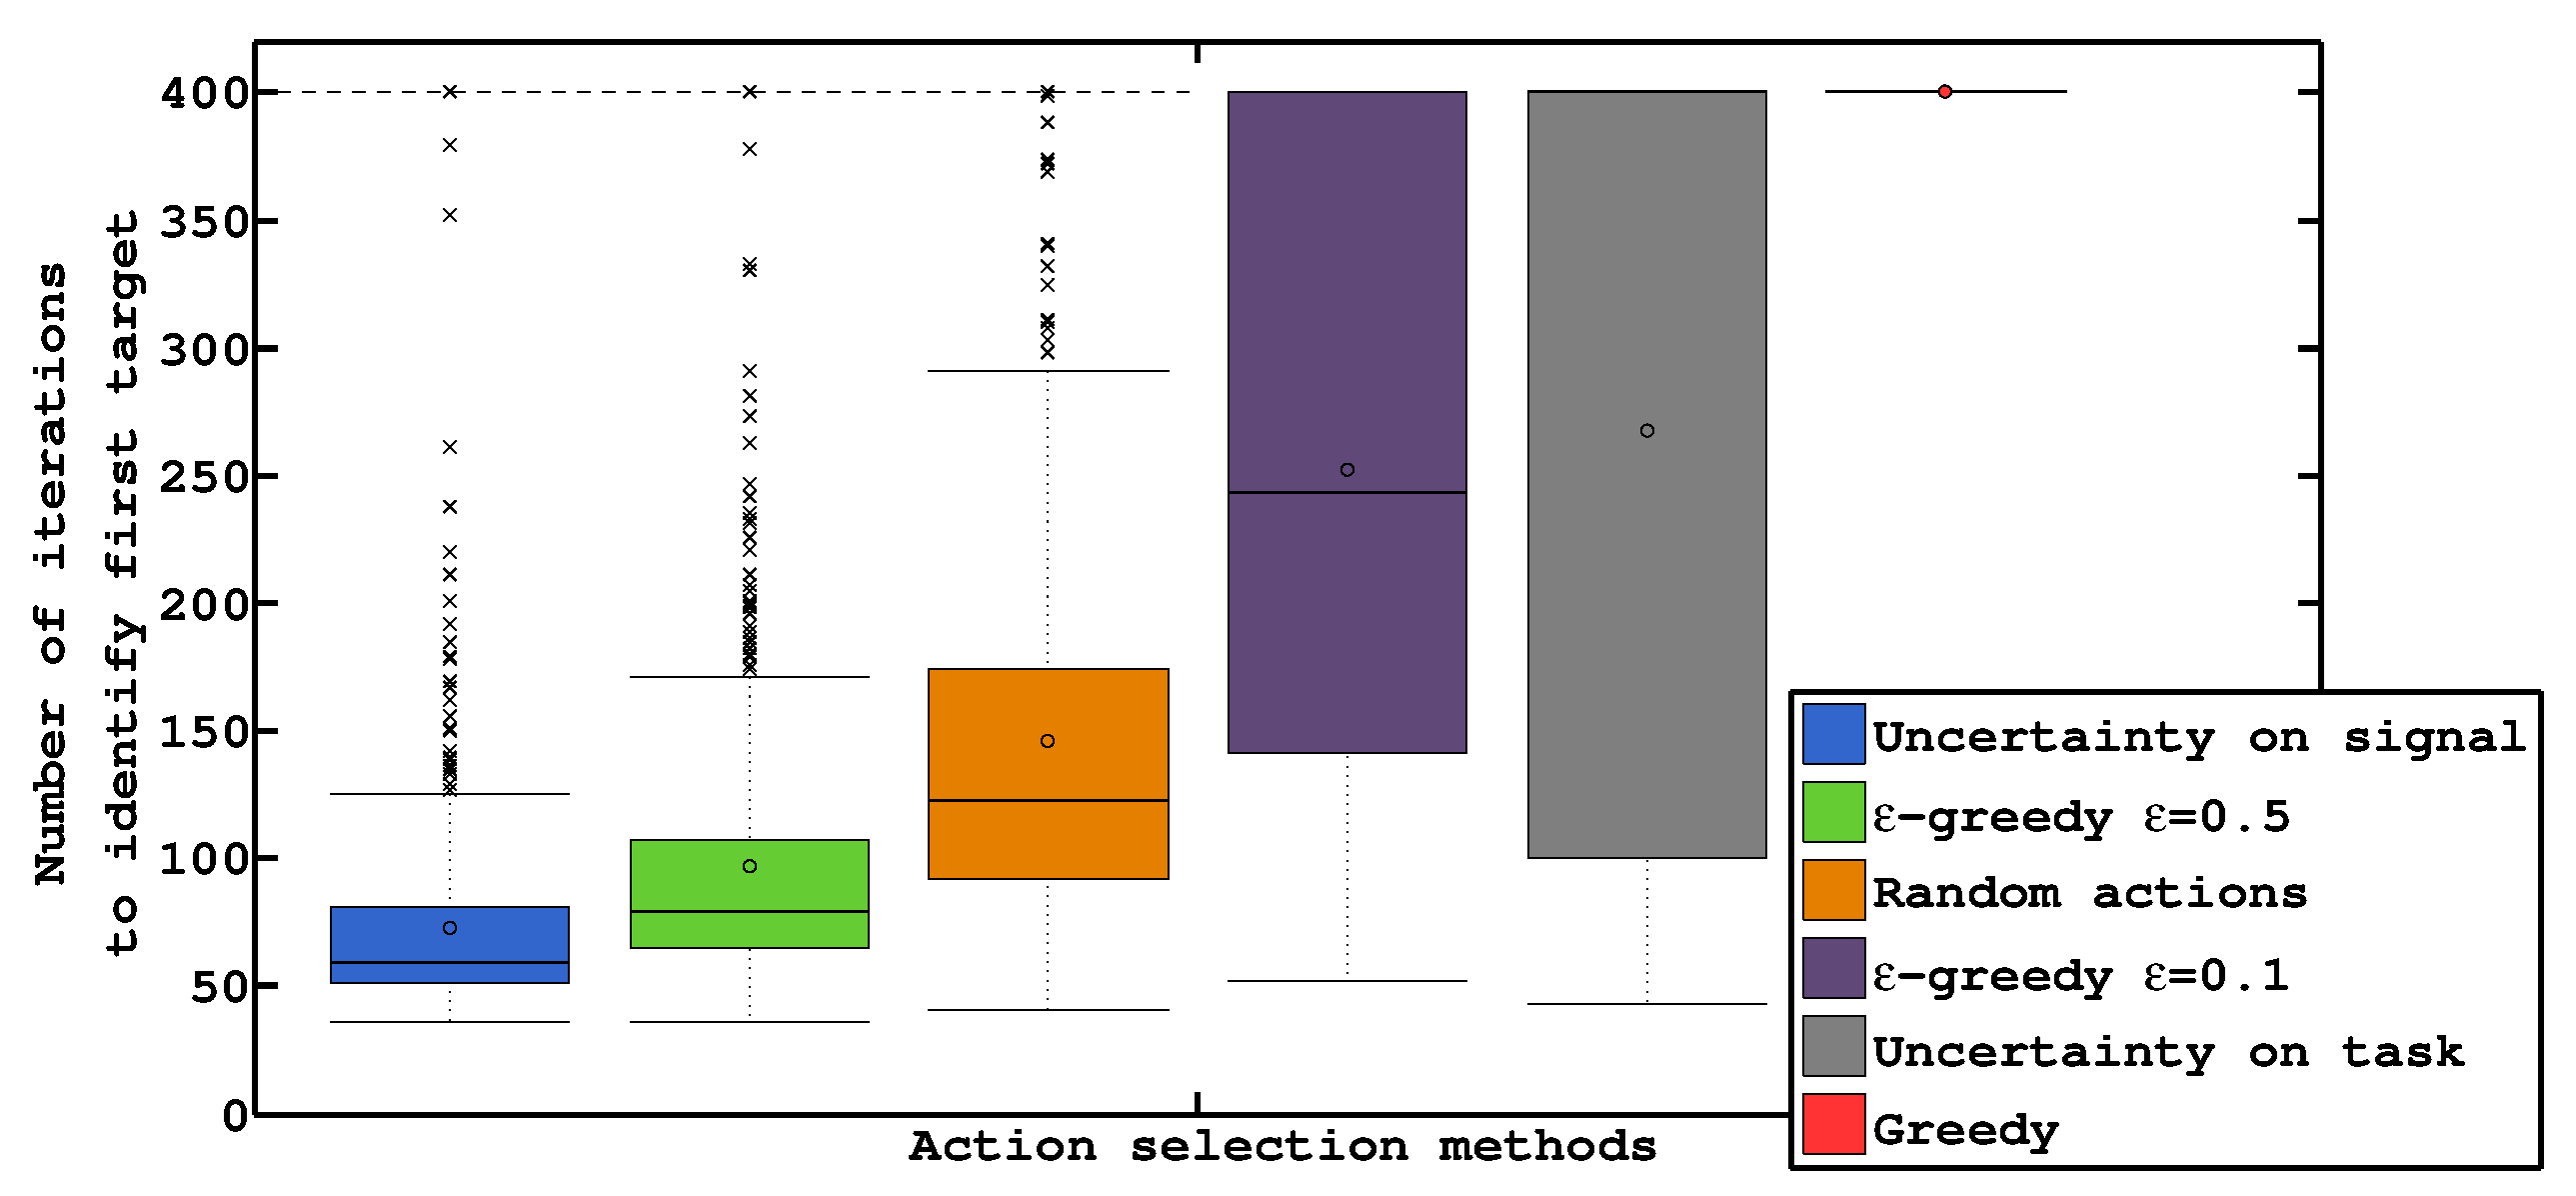
\includegraphics[width=\columnwidth]{img/plot_planning_first}
    \caption{Comparison of different exploration methods. Our proposed method, based on the uncertainty on the task and the signals interpretation, allows to lead the system to regions that improve disambiguation among hypotheses in a faster way. For the greedy method, all values were $400$ which indicates it never allowed to identify any task.}
    \label{fig:compplan}
\end{figure}

Figure~\ref{fig:compplan} shows the results averaged across subjects, runs and datasets. Values of $400$ means the confidence threshold was not reached after 400 iterations. Our proposed method, based on the uncertainty on the task and the signals interpretation, allows to lead the system to regions that improve disambiguation among hypotheses in a faster way. Trying to follow the most probable task does not allow the system to explore sufficiently (Greedy), and at least some random exploration is necessary to allow a correct identification of the task ($\varepsilon$-greedy). Assessing uncertainty only on the task performs poorly as it does not take into account the signal interpretation ambiguity inherent to our problem. The large variability in the results is mainly due to the large variations in classification accuracy across subjects and datasets. Given these results, the remainder of this section will only consider our proposed planning method.

\paragraph{Online re-estimation of classifier}
After identifying the first task, and following our approach, we continued running the system and measured how many tasks were identified after $400$ steps. The quality of our unsupervised method can be measured according to the percentage of labels correctly assigned (according to the ground truth label), see Figure~\ref{fig:percentageLabels}. In general, having dataset with classification accuracies higher than $75\%$ guaranteed that more than $90\%$ of the labels were correctly assigned. This result shows that our algorithm can also be used to collect training data for calibrating any other state-of-the-art error-related potentials classifier, but has the important advantage of controlling the device at the same time.

\begin{figure}[!ht]
    \centering
        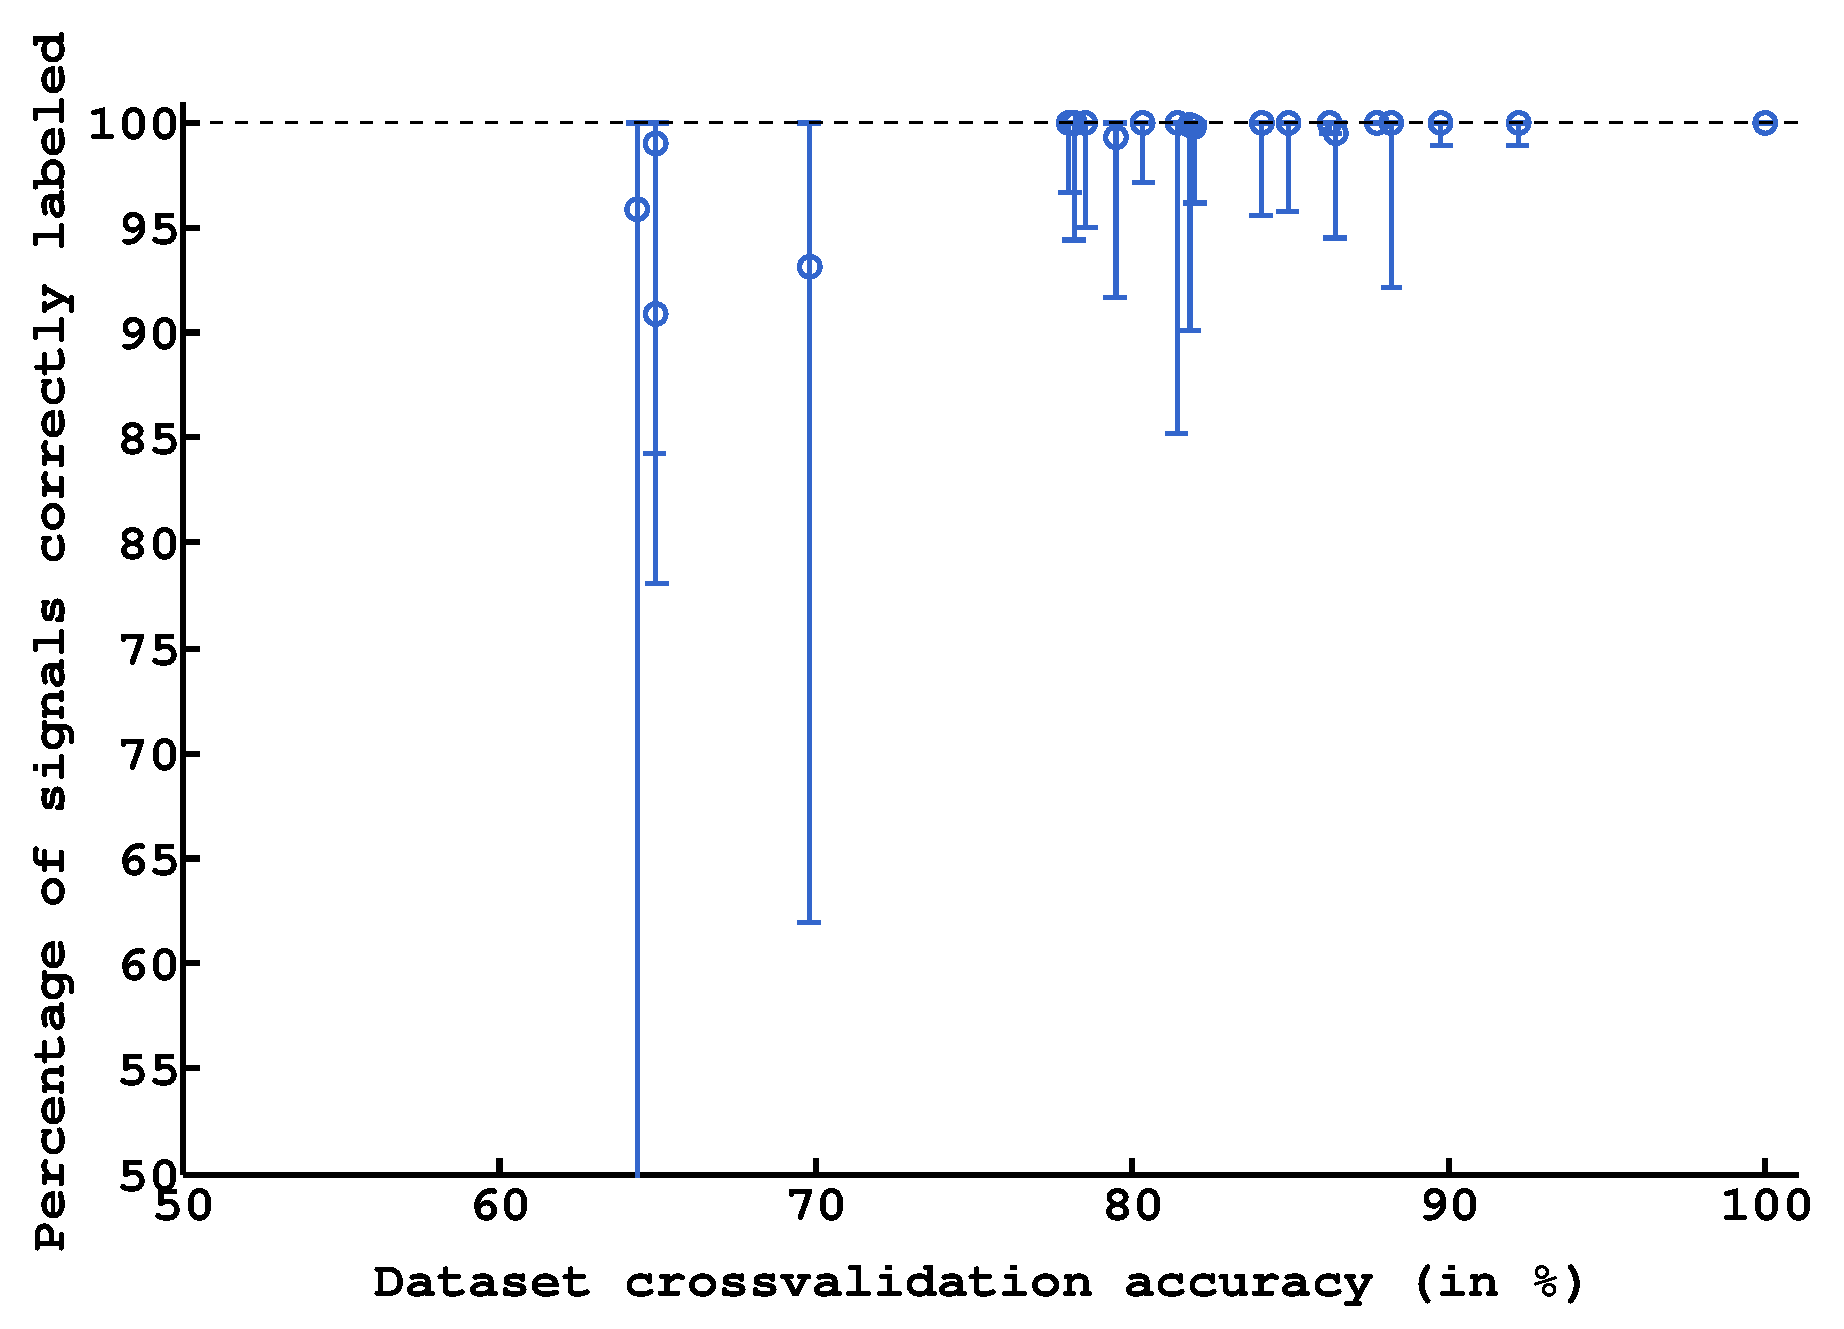
\includegraphics[width=\ww\columnwidth]{img/plot_percent_label}
        \caption{Percentage of labels correctly assigned according to the ground truth label (the markers show the median values and the error bars the $2.5$th and $97.5$th percentiles). In general, having dataset with classification accuracies higher than $75\%$ guaranteed that more than $90\%$ of the labels were correctly assigned.}
        \label{fig:percentageLabels}
\end{figure}

Figure~\ref{fig:bhatta} demonstrates the advantage of switching to a Bayes filter method after identification of a first target instead of keeping the estimation given by the Bhattacharyya coefficient. On the one hand, Bhattacharyya coefficient works very well for small amounts of data because it directly compares model parameters. On the other hand, when there is sufficient data, training a classifier allows for a faster identification since the classifier makes a much harder decision when evaluating a new EEG signal.

\begin{figure}[!ht]
    \centering
        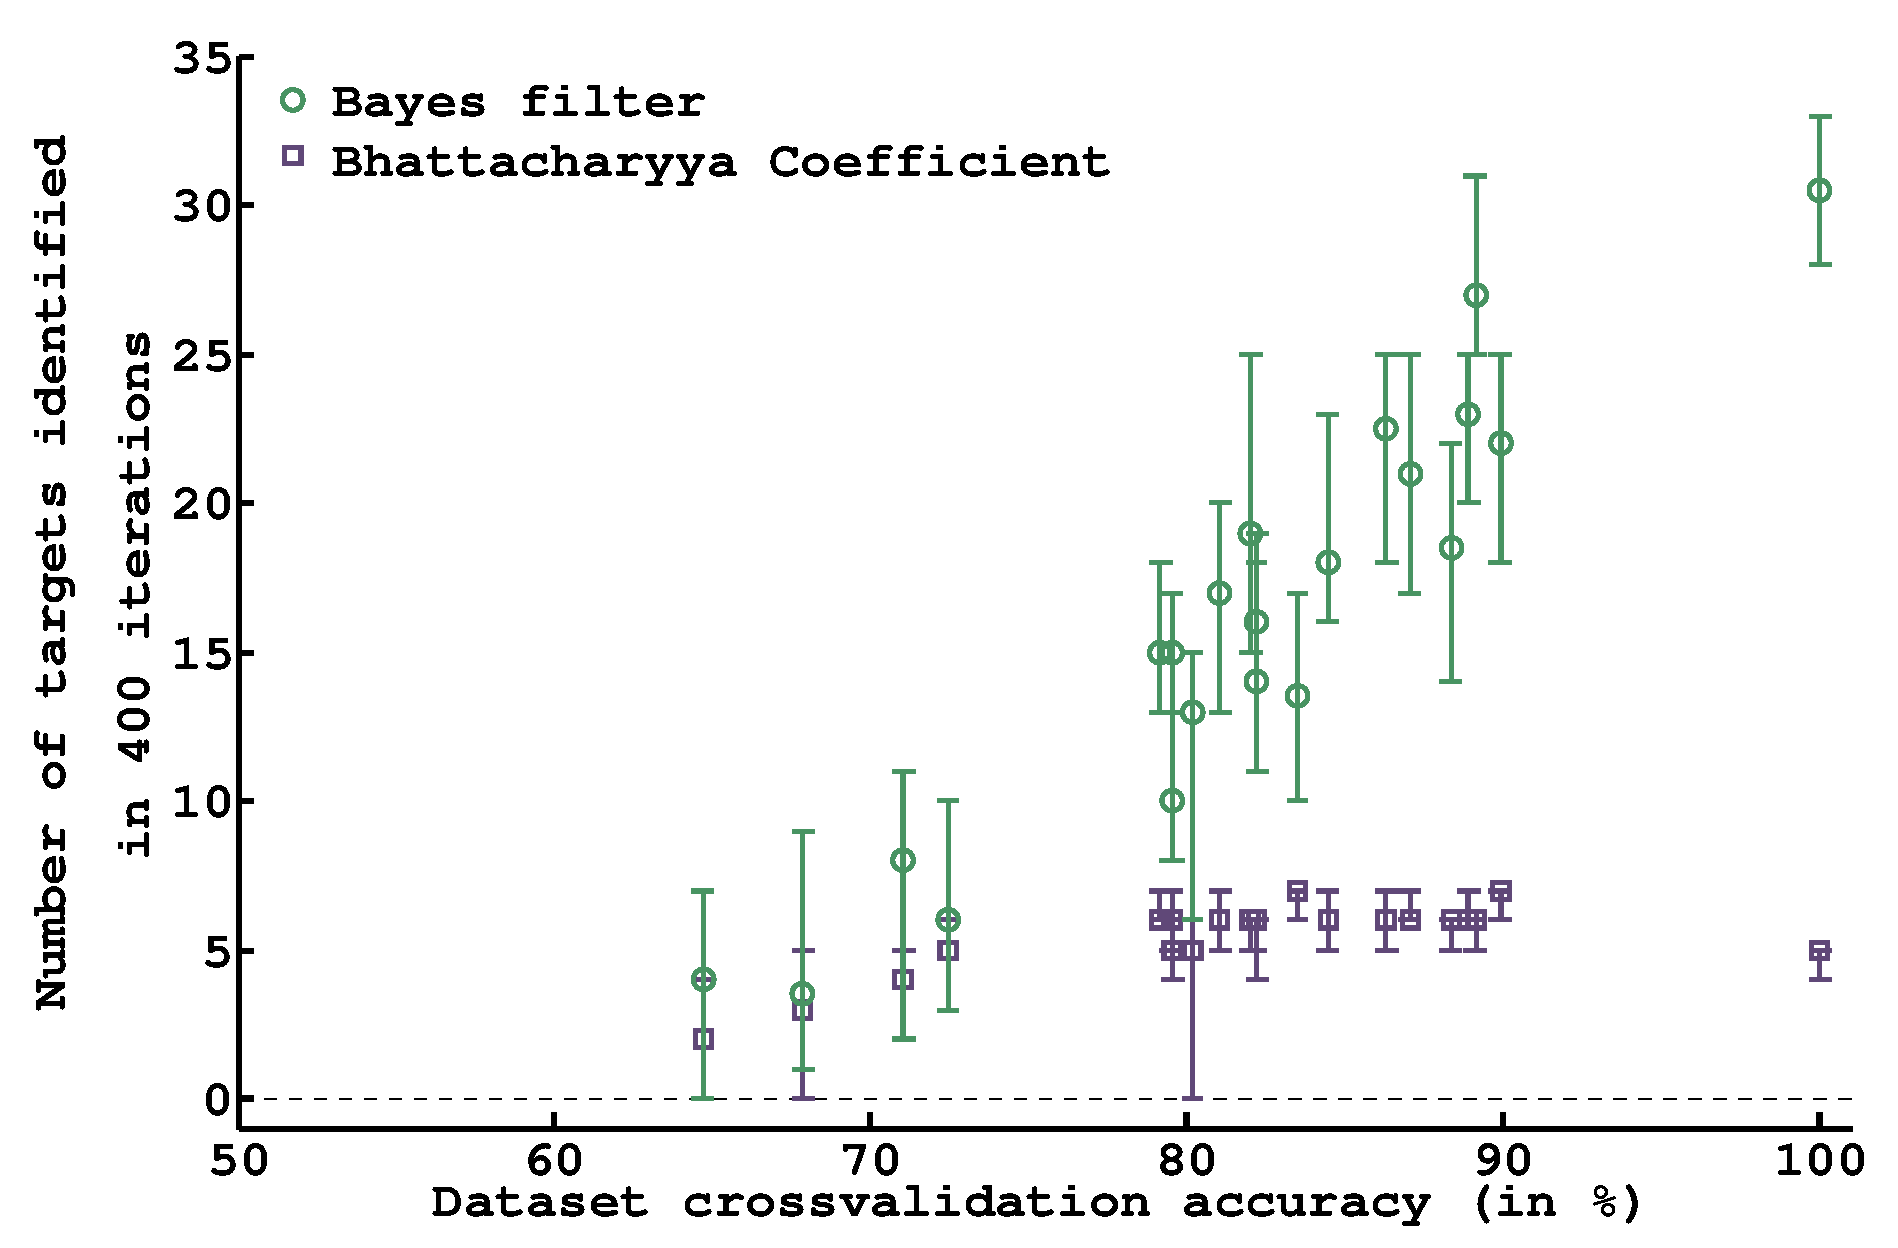
\includegraphics[width=\ww\columnwidth]{img/plot_bhattha_vs_bayes}
        \caption{Number of targets correctly identified in $400$ iterations (the markers show the median values and the error bars the $2.5$th and $97.5$th percentiles). Comparison between switching to a Bayes filter method after identification of a first target instead of keeping the estimation given by the Bhattacharyya coefficient. The Bayes filter allows for a faster identification.}
        \label{fig:bhatta}
\end{figure} 

Figure~\ref{fig:avg_sum_400} shows the number of tasks correctly and incorrectly identified in $400$ iterations. For datasets of good qualities, we are able to identify more than $20$ tasks in $400$ iterations without the need for a calibration procedure (recap that previous works needed between 300 and 600 examples for the calibration phase \cite{chavarriaga2010learning,iturrate2010single}). The number of correctly identified tasks is strongly correlated to the quality of the dataset.

\begin{figure}[!ht]
    \centering
    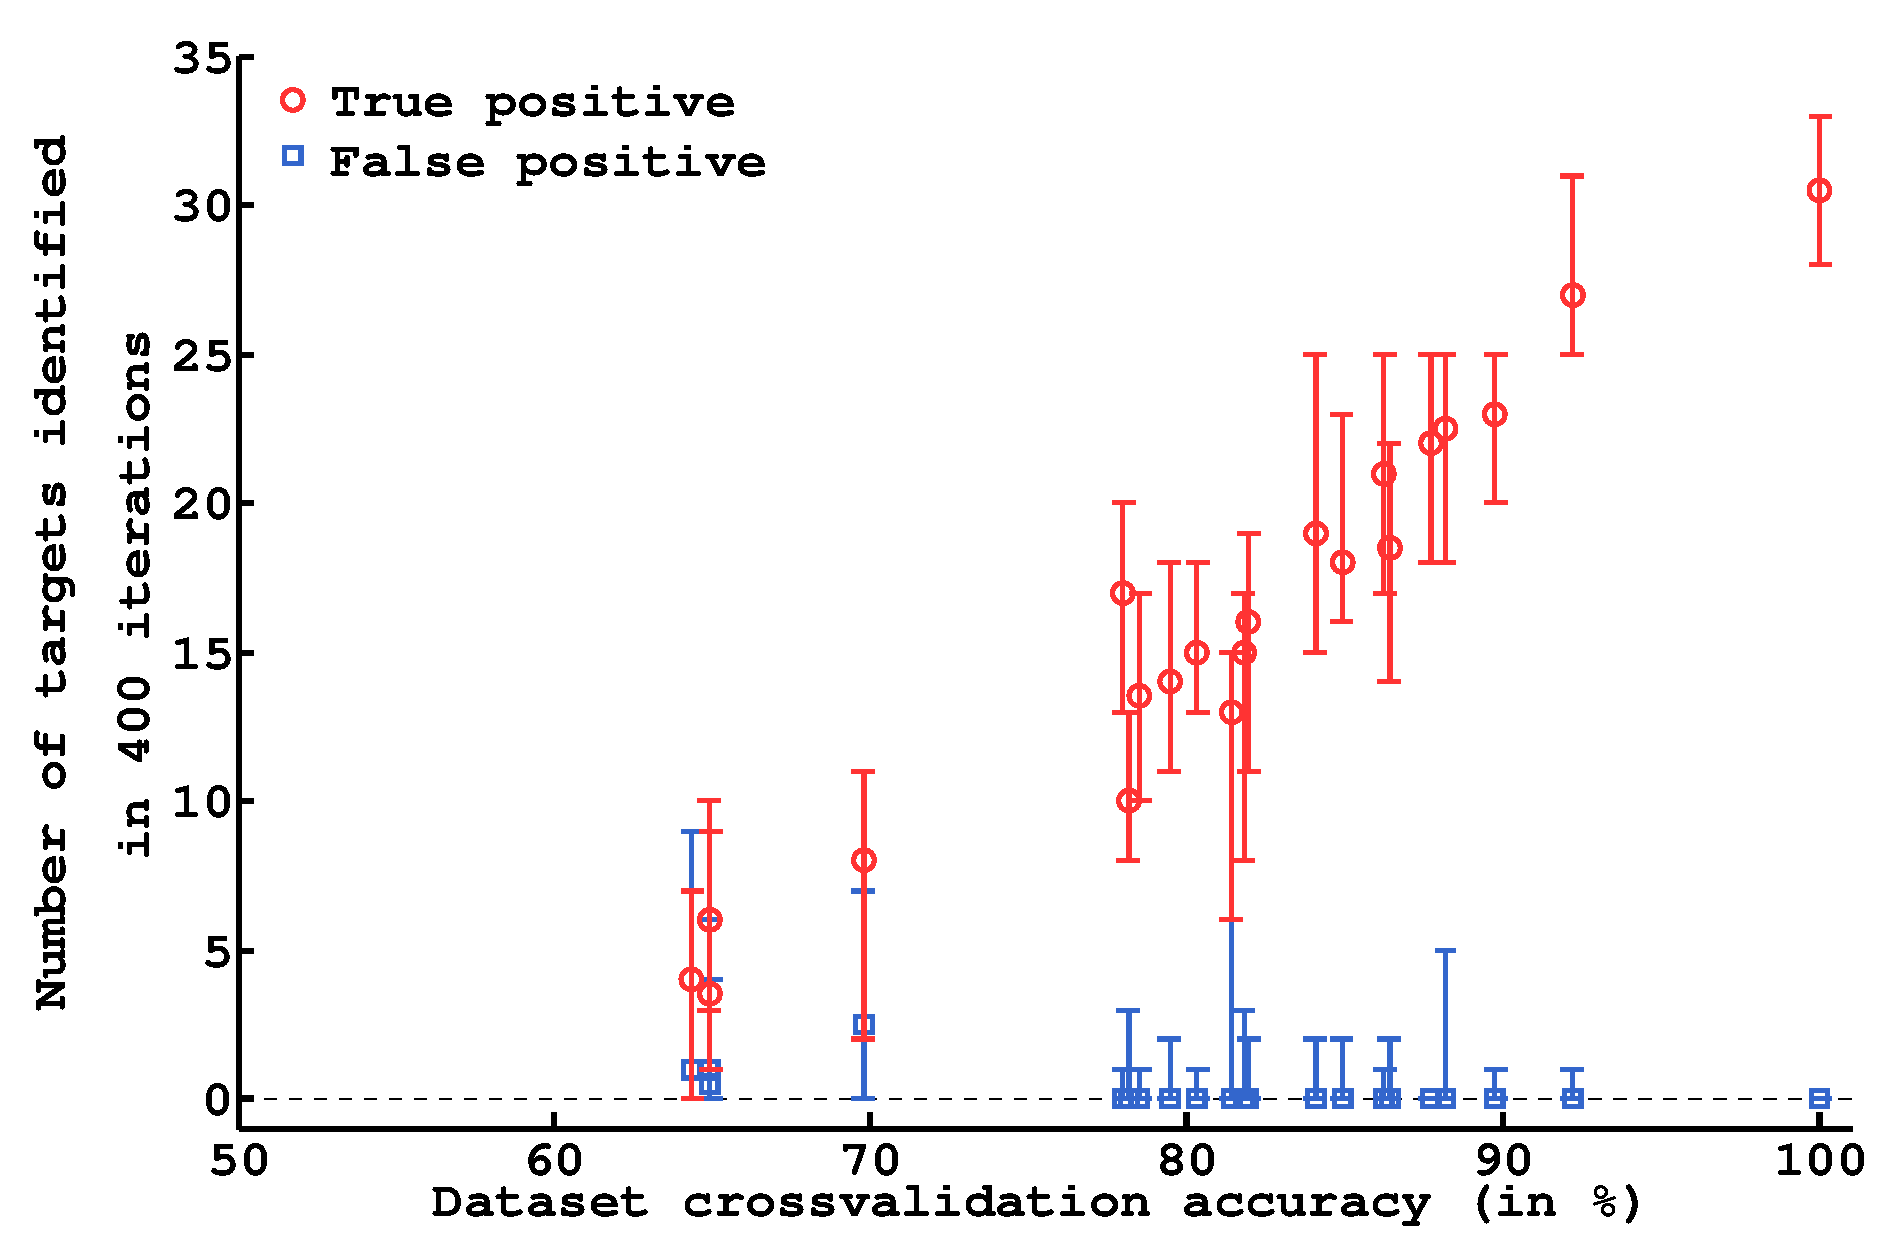
\includegraphics[width=\ww\columnwidth]{img/plot_first400_reach} 
    \caption{Number of targets correctly and incorrectly identified in $400$ iterations (the markers show the median values and the error bars the $2.5$th and $97.5$th percentiles). For datasets of good qualities, we are able to identify more than $20$ tasks in $400$ iterations without the need for a calibration procedure.}
    \label{fig:avg_sum_400}
\end{figure} 

\paragraph{Robustness to Abrupt Changes in the Signals' Properties }
\label{CenterRobustnessToAbruptChangesInTheSignalsProperties}

We now want to determine whether the system is robust to changes in the signals' properties that occur when we change between different problem settings \cite{IturrateErrP13}. We modeled this by changing from $Ti$ to $Tj$ ($i \neq j$) after $400$ steps, and then executing $400$ more steps from $Tj$. Both combinations ($T1$ to $T2$ and $T2$ to $T1$) were tested.

Figure~\ref{fig:stage2} shows the number of tasks identified depending on the classification accuracy on $Tj$ when training a classifier from dataset $Ti$. For abrupt changes which conserve a classification accuracy above $70\%$ on the new signals, our method, based on a limited size prior, is able to recover and solve more than $20$ tasks in $400$ iterations. For those cases where the accuracy change is too drastic, starting from scratch may be a better solution than relying on the adaptation properties of our algorithm.

\begin{figure}[!ht]
    \centering
    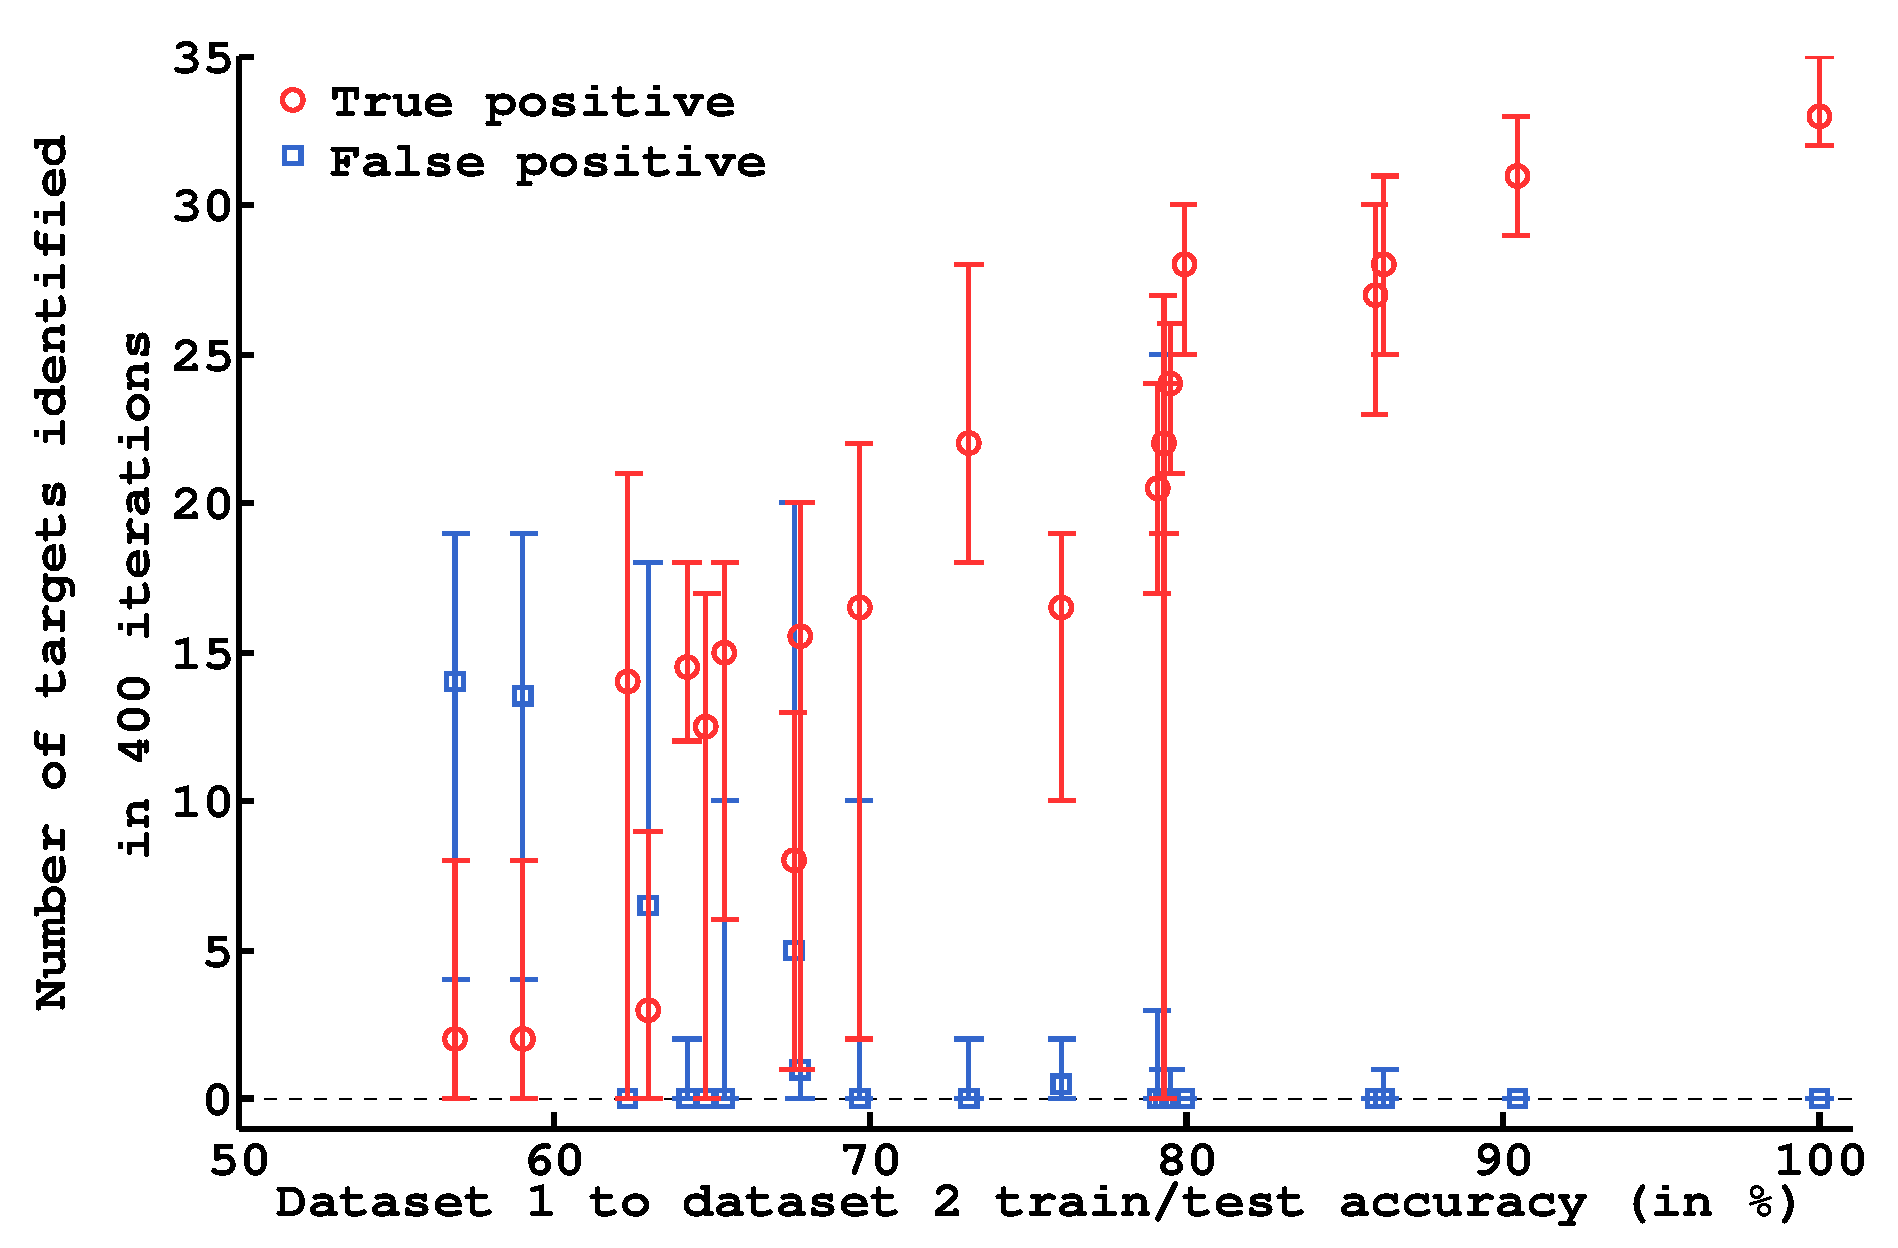
\includegraphics[width=\ww\columnwidth]{img/plot_last400_reach}
    \caption{Number of targets correctly and incorrectly identified in $400$ iterations after an abrupt change in the signals properties (the markers show the median values and the error bars the $2.5$th and $97.5$th percentiles). For abrupt changes which conserve a classification accuracy above $70\%$ on the new signals, our method, based on a limited size prior, is able to recover and solve more than $20$ tasks in $400$ iterations.}
    \label{fig:stage2}
\end{figure}

\section{Conclusion}

We introduced a novel method for calibration-free BCI based control of sequential tasks with feedback signals. The method provides an unsupervised way to train a decoder with almost the same performance as state-of-the-art supervised classifiers, while keeping the system operational and solving the task requested by the user since the beginning. 
%
The intuition for our method is that the classification of the brain signals is easier when they are interpreted according to the task desired by the user. The method assumes a distribution of possible tasks and relies on finding which pair of decoder-task has the highest expected classification rate on the brain signals. 


The algorithm was tested with real online experiments, showing that the users were able to guide an agent to a desired position by mentally assessing the agent's actions and without any explicit calibration phase. Offline experiments show that we can identify an average of 20 tasks in 400 iterations without any calibration, while in previous works the calibration phase used between 300 and 600 examples. To improve the efficiency of the algorithm, we introduced a new planning method that uses the uncertainty in the decoder-task estimation. Finally, we analyzed the performance of the system in the presence of abrupt changes in the EEG signals. Our proposed method was able to adapt and reuse its learned models to the new signals. Furthermore, in those cases when the transfer is not possible, our method can still be used to recalibrate the system from scratch while solving the task.

A current limitation of the work is the need for a finite set of task hypotheses. This limitation could be solved by the use of a combination of particle filter and regularization on the task space. Additionally, our method can not dissociate fully symmetric hypotheses, e.g.\ right and left most state of our 1D grid world (Fig. \ref{fig:GM}), as the interpretation of feedback signals will also be symmetric and therefore as likely. This latter problem can be solved by redefining the set of hypotheses or the action set, for instance by adding a ``stop'' action valid only at the target state.

This work opens a new perspective regarding the global challenge of interacting with machines. It has application to many interaction problems which requires a machine to learn how to interpret unknown communicative signals. A promising avenue, outside the BCI field, lies in human robot interaction scenarios where robots must learn from, and interact with, many different users who have their own limitations and preferences.

\section{Acknowledgments}
The authors would like to thank the anonymous reviewers for their helpful comments which contributed in improving the quality of this paper. The authors from INRIA are with the Flowers Team, a join INRIA - Ensta ParisTech lab, France. Luis Montesano is with Instituto de Investigaci\'{o}n en Ingenier\'{i}a de Sistemas, Universidad de Zaragoza, Spain. I\~{n}aki Iturrate is with the Chair in Non-invasive Brain-Machine Interface (CNBI) and Center for Neuroprosthetics and Institute of Bioengineering, EPFL, Switzerland. This work has been partially supported by INRIA, Conseil R\'egional d'Aquitaine and the ERC grant EXPLORERS 24007; and from the Spanish Ministry via DPI2011-25892 (L.M.), and DGA-FSE grupo T04.

\begin{quote}
\begin{small}
\bibliographystyle{aaai}
\bibliography{grizou}
\end{small}
\end{quote}

\end{document}
